\documentclass{article}

\usepackage[utf8]{inputenc} 
\usepackage{outlines}
\usepackage{amsmath}
\usepackage{cleveref}
\usepackage{graphicx}
\usepackage{xr}
\usepackage{siunitx}

\usepackage[margin=1in]{geometry}
\parskip 1.5ex % paragraph spacing

\graphicspath{./docs/Figures/}

\title{Temp RM}
\author{Tom}
\date{January 2021}

\begin{document}

\maketitle

\section{Introduction}

Temperature has long been recognised as a fundamental environmental driver in ecology (REF). It's effects are felt across multiple scale of organisation from individual physiology (REF) to the dynamics of whole communities and ecosystems (REF) and are visible in the natural temperature gradients that shape ecosystems across both time (e.g. seasonal fluctuations) and space (e.g. latitudinal or elevations gradients)(REF). Temperature is also becoming increasingly relevant as an environmental driver as rates of global warming continue to increase, a process which is predicted to have large consequences for ecosystems and their functioning in the future (REF). Thus, it is clear that we need to understand the mechanisms through which temperature affects ecosystems, given both how ubiquitous its effects are and the need to understand and predict the effects that future warming may have. 

One aspect of temperature that is particularly important is how it affects ecosystem dynamics, the process through which the structure of ecosystems change over time (REF). Ecologists have long been interested in ecosystem dynamics, especially in what they tell us about the ability of ecosystems to persist though time and respond to environmental perturbations (such as temperature)(REF). Though stability, defined as the ability of system to return to some state following a perturbation (REF), has been the focus of much of this research, a whole host of other dynamical measures have also been defined such as reactivity (the strength of the initial response of an ecosystem to a perturbation; REF), resilience (the asymptotic rate of return to equilibrium following a perturbation) and feasibility, which we focus on here. 

An ecosystem is defined to be feasible if there exists a fixed point at which all populations within have positive biomass, that is, all species in the system are able to coexist at equilibrium (REF). Feasibility has recently been highlighted as an important ecosystem property due its role as a prerequisite for other aspects of ecosystem dynamics (e.g. stability, resilience, and reactivity mentioned above). This is because by definition, only the properties of fixed points that actually exist (i.e those guaranteed by the feasibility of systems) are relevant to ecosystem dynamics (REF) or in other words, a system must be feasible in the first place for many of these other dynamic measures to have meaning. Recent work has revealed the importance of species' functional traits (e.g. growth rates and interactions) in determining feasibility, showing how the feasibility condition places a constraint on these trait values within ecosystems. Importantly this work has also linked the feasibility of systems to the number of species they contain (REF) which combined, suggest that we may be able use feasibility as a way to explore patterns of species richness and link them to species traits (REF). 

Though no previous work has looked directly at the relationship between feasibility and temperature, there have been other attempts to understand the thermal responses of whole ecosystem properties(REF). Broadly this work has tended to use the simplifying assumption of constant temperature dependence, that all populations and traits have the same response to temperature. This allows the derivation of simple analytic predictions which often show a single monotonic (i.e. strictly increasing or decreasing) temperature response (REF). However, this approach has been met with criticism due to both work demonstrating widespread variation in thermal sensitivity of across different demographic processes and taxa and the evidence showing that many of these properties actually demonstrate uni-modal (i.e. peaked) thermal responses. Furthermore a growing body of work shows how important this variation in thermal responses (often referred to as "mismatches") can be in determining the dynamics a number of ecological contexts such as of predator-prey (REF), and virus (REF) and parasite-host (REF)  systems.  

In this paper we investigate the relationship between temperature, feasibility and its impact of the species richness in ecosystems. Broadly our approach is to utilise the previously identified relationship between feasibility and population demographic parameters (growth rates and interactions) which themselves are expected to have a temperature dependence due their dependence on metabolic rate (REF). In this way we can metabolically constrain the response of these traits to temperature and thus derive predictions regarding the temperature dependence of ecosystem feasibility and species richness. Crucially our approach differs from previous work looking at the temperature dependence of ecosystem level properties, allowing us to account for variation in their thermal response of different traits and populations within the ecosystem. Ultimately this lets us consider the effects of such variation on feasibility and species richness and provides mechanistic insight into the relationship of ecosystem dynamics with temperature.

\section{Theory}
\subsection{The mean-field model}
In order to explore feasibility and its temperature dependence we use the generalised Lottka-Volterra model (GLV) (REF). This framework is commonly used to explore ecosystem dynamic properties and is regularly applied to study complex, multi-species communities (REF). The GLV describes the dynamics of an $N$ species system where the growth of species $i$ is given by:

\begin{equation} \label{EQ:GLV}
  \frac{1}{x_i} \frac{dx_i}{dt} = r_i - a_{ii} x_i - \sum^N_{i \neq j} a_{ij} x_j, 
\end{equation}

where $x_i$ is the biomass of the $i$th species, $r_i$ is it's intrinsic growth rate, determining the rate at which new biomass is produced ($\text{mass} \cdot \text{time}^{-1} \cdot \text{mass}^{-1} $) and $a_{ij}$ describes the effect of interactions with species $j$ on $i$ (with the $a_{ii}$ term representing intraspecific interactions; $\text{mass}^{-1} \cdot \text{time}^{-1}$). As we want to determine the feasibility of this system (i.e. whether the system will support non-zero biomasses for all species at equilibrium) we need to derive an expression for the equilibrium biomasses. Though it is not possible to derive an exact analytical solution for the GLV as described in \cref{EQ:GLV}, we can use a mean-field approximation, developed by (REF) to get estimate of equilibrium biomass (\cref{SI_Sec:Meanfield}). This approximation works by considering interaction term from \cref{EQ:GLV}, which we can rewrite as:

\begin{equation} \label{EQ:mean_int} 
    \sum^N_{i \neq j} a_{ij} x_j = (N-1) \bar{a x} = (N-1) \bar{a} \bar{x} + (N-1) \text{cov}(a,c),
\end{equation}

where the bar notation, $\bar{\cdot}$, represents the average of that quantity over all $N$ species in the system. \Cref{EQ:mean_int} partitions the effects of interactions on the $i$th species into the average effect across the system, $\bar{a} \bar{x}$, and the covariance between heterospecific's biomass and the strength of interactions, $\text{cov}(a,x)$. The mean-field approximation assumes that this second term is negligible, which is equivalent to saying that any individual interaction between the focal species and another species population has little effect on that heterospecific's biomass. We also assume here that the system we consider is large ($N \gg 0$), meaning that the difference between the average biomass across the system and that of heterospecifics is small (as it is in the order $N^{-1}$) and can thus be ignored. For simplicity we make the further assumption that intraspecific interactions are constant across species, setting $a_{ii} = 1$ (though this assumption can be relaxed for the mean0field approximation (REF)). Combining \cref{EQ:GLV,EQ:mean_int} we can then express population dynamics in terms the average interaction strength, giving the full mean-field model:

\begin{equation} \label{EQ:MF}
    \frac{1}{x_i} \frac{dx_i}{dt} \approx r_i - x_i - (N-1)\bar{a}\bar{x}.
\end{equation}

By setting \cref{EQ:MF} equal to $0$ and solving for $x_i$ we then obtain an expression for equilibrium biomass (see \cref{SI_Sec:Meanfield}):

\begin{equation}\label{EQ:MF_eqi}
  x^*_i \approx K_i -  \bar{K}  \frac{ (N-1)\bar{a}}{1 + (N-1)\bar{a}}, 
\end{equation}

where $K_i = \frac{r_i}{a_{ii}}$ is the carrying capacity, the biomass a population would reach if grown in isolation (obtained by solving \cref{EQ:MF} with $\bar{a} = 0$). \Cref{EQ:MF_eqi} provides an intuitive expression for the equilibrium biomasses; a species is expected to reach the biomass that it would in isolation (first term of the RHS, $K_i$) minus the effects of any interspecific interactions (second term on RHS). The strength of these interspecific effects is determined by the average carrying capacity of heterospecifics ($\bar{K}$) and a saturating function of interactions experienced by the focal species, $(N-1)\bar{a}$. If interactions are overall competitive (i.e. $ \bar{a} > 0$) then we see a reduction in equilibrium biomass relative to the individual carrying capacities whereas if they are facilitatory ($ \bar{a} < 0$) we see an increase.  

\subsection{Feasibility} \label{Sec:Feasibility}
We use \Cref{EQ:MF_eqi} to derive an expression for the feasibility of a system in terms of the population demographic parameters (i.e. the $r_i$'s and $a_{ij}$'s). We start by recalling that a system is feasible if all species have non-zero equilibrium biomass (i.e. $x_i^* > 0 $), giving the condition:

\begin{align} \label{EQ:Feas_sp}
  \kappa_i > \frac{(N-1)\bar{a}}{1 + (N-1)\bar{a}} \quad \text{for all} \quad i = 1 \ldots N,
\end{align}

where $\kappa_i = \frac{K_i}{\bar{K}}$ is the mean-normalised carrying capacity. \Cref{EQ:Feas_sp} shows how a system is feasible as long as the the effects of interspecific interactions on the each population (RHS) do not outweigh the effects of intraspecific interactions (LHS). We can see that in the case of facilatory interaction ($\bar{a} < 0$) the inequality will always hold and the system will be feasible. Only when interactions are on average competitive (i.e $\bar{a} > 0$) will systems be unfeasible. 

\subsubsection{Probability of Feasibility}

Using \cref{EQ:Feas_sp} we can also formulate an expression for the probability of feasibility $P_{feas}$, the chance that an ecosystem is feasible given the distribution of species trait values ($\kappa$s and $a$s) and number of species in the system. To do so we take \cref{EQ:Feas_sp} and consider $\kappa$ and $a$ as random variables, each describing the distribution of the respective traits across the community (represented in notation by the loss of subscript). This lets us consider $\kappa$'s cumulative density function (CDF) which gives the probability that $\kappa$ is less than or equal to some value, $F_{\kappa}(x) = P(\kappa \leq x)$. As the condition for feasibility states that $\kappa$ must be greater than the effect of interactions we can apply the CDF to \cref{EQ:Feas_sp} and write $P_{feas}$ as:

\begin{equation} \label{EQ:P_feas}
    P_{feas} = P \left( \kappa > \frac{(N-1)\bar{a}}{1 + (N-1)\bar{a}}  \right)^N = 
    \left[1 - F_{\kappa}\left(\frac{(N-1)\bar{a}}{1 + (N-1)\bar{a}}\right)\right]^N,
\end{equation}

giving the probability of feasibility of an ecosystem as a function of the species traits (\cref{Fig:P_feas}). Note the expression is raised to the $N$th power as the term in the brackets must hold for all $N$ populations in the system for it to be feasible. 

\begin{figure}
    \centering
    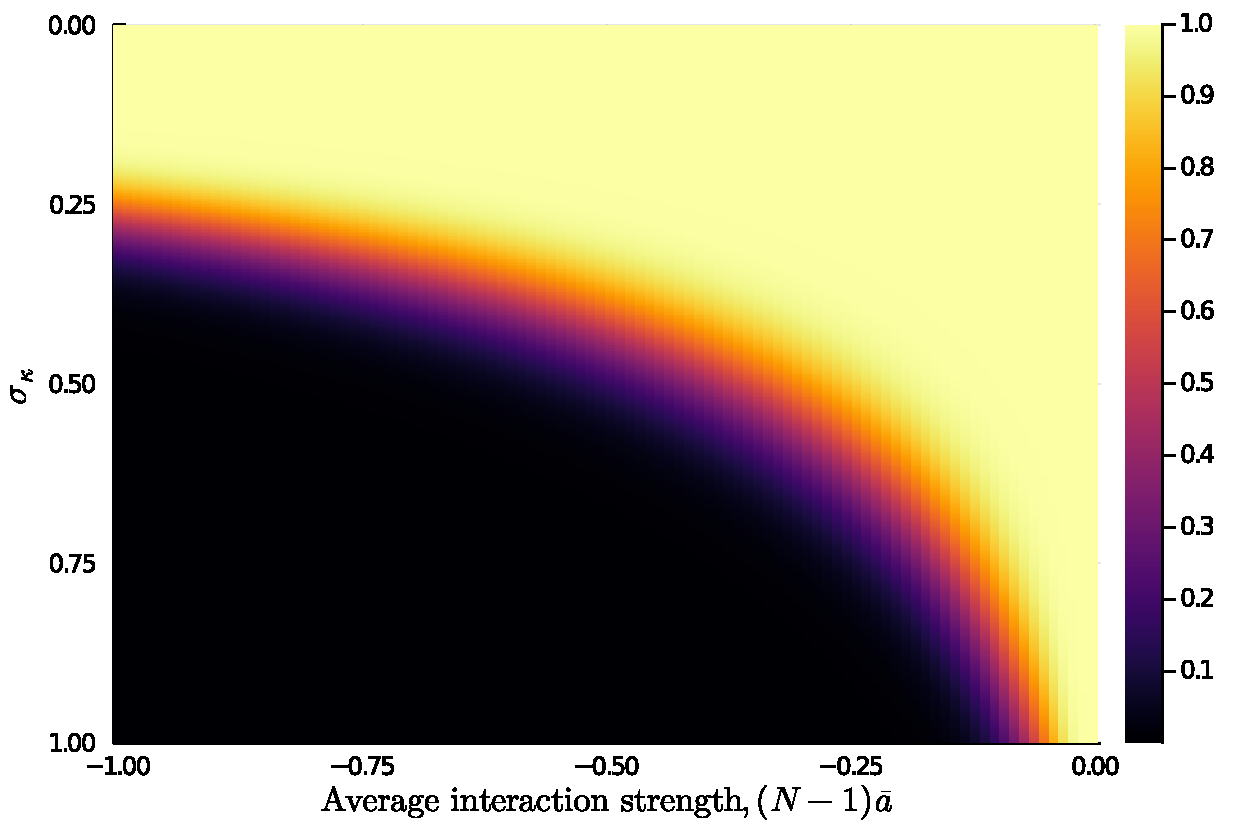
\includegraphics[width = 0.6\textwidth]{docs/Figures/Fig_2.pdf}
    \caption{\textbf{The probability of feasibility $P_{feas}$ as a function of interaction strength and variation in normalised carrying capacity $\sigma_{\kappa}$}. Feasibility shows the same general pattern as \cref{Fig:Feasability_Bound}, decreasing as interactions become more negative and as the variation in $\kappa$ increases (reducing the chance that all species meet the criteria in \cref{EQ:Feas_sp}). $P_{feas}$ is calculated using \cref{EQ:P_feas} setting $N=50$ and allowing $\sigms_{\kappa}$ and $\bar{a}$ to vary such that $\sigma_{\kappa} \in [0 - 1]$ and $\bar{a} \in [-1 - 0]$}
    \label{Fig:P_feas}
\end{figure}

\subsection{Temperature} \label{SEC:Temperature}
In order to relate the conditions for feasibility to temperature we consider how temperature affects the parameters in \cref{EQ:P_feas}, the normalised carrying capacities $\kappa$ (driven here primarily by changes in population growth rate $r$), and inter-species interactions $a$. There is a large body of empirical and theoretical work demonstrating the existence and consequences of the temperature dependence of these processes which can be explained by their dependence on metabolic rate (REF). This determines the capacity of individuals to fuel growth and interactions which in turn is affected by temperature through its effects on biochemical kinetics (REF).

We use the modified Boltzmann-Arrhenius equation to represent the temperature dependence of $\kappa$ and $a$, which describes the exponential-like increase of some process with temperature (REF). Though empirically measured temperature response curves tend to have a uni-modal shape, we use the Boltzmann-Arrhenius due to its analytic tractability and its ability to capture the rising portion (before the temperature peak) of these curves. We focus on this part of the curve as it is expected that the range of temperatures individuals actually experience (their operational temperature range) tends to below this thermal peak, making the exponential portion more relevant for the dynamics of real ecosystems (REF). This form of the Boltzmann-Arrhenius uses two parameters to describe the thermal response of a some process $B(T)$, the normalisation constant $B_0$ which is the value at a reference temperature and thermal sensitivity $E$ which determines the magnitude of the response of $B(T)$ to changes in temperature:

\begin{equation} \label{EQ:Boltzmann}
    B(T) = B_0 e^{-\frac{E}{k} \left(\frac{1}{kT} - \frac{1}{k T_{ref} }\right)},
\end{equation}

where $k$ is the Boltzmann constant and $T$ and $T_{ref}$ are the temperature and reference temperature (in kelvin) respectively. Applying \cref{EQ:Boltzmann} allows us to characterise the distributions of parameters across species populations at different temperatures in terms of the distributions of the underlying thermal sensitivity parameters ($B_0$s and $E$s), instead of having to define them directly. Assuming that the parameter values follow a log-normal distribution (a natural assumption given the exponential form of \cref{EQ:Boltzmann}), we obtain an expression for the temperature dependent distribution of $B(T)$ (see \cref{SI_Sec:TPC_dist}):

\begin{align} \label{EQ:Boltz_dist}
    \log(B(T)) \sim \mathcal{N}\left(\mu_{B}(T) , \sigma_{B}^2(T) \right) 
    \quad \text{where} \quad
    \begin{array}{cc}
        \mu_B &= \mu_{B_0} - \mu_{E} \left(\frac{1}{kT} - \frac{1}{k T_{ref} }\right)  \\
        \sigma_{B}(T)^2 &= \sigma_{B_0}^2 + \sigma_{E}^2 \left(\frac{1}{kT} - \frac{1}{k T_{ref} }\right)^2
    \end{array}
\end{align}

where $\mu$ and $\sigma^2$ represent the mean and variance respectively. \Cref{EQ:Boltz_dist} makes explicit the effect of thermal sensitivity parameters on the distribution of $B(T)$ showing that the sign and magnitude of the temperature response is controlled mainly by the average thermal sensitivity, $\mu_E$, as a linear function of temperature with the variance introducing an additional quadratic term which creates curvature in the thermal response. The distribution of normalisation constants $B_0$s is present simply as an constant term in the expressions for both mean and variance. It is important to note here that as $B(T)$ is log-normally distributed it's moments are defined in terms of both the mean and variance in \cref{EQ:Boltz_dist} and thus both factors (the linear and quadratic parts) will contribute to the shape of the distribution. Applying \cref{EQ:Boltz_dist} to the distributions of $\kappa$ and $\bar{a}$ we obtain the expressions:

\begin{align} \label{EQ:Trait_distributions}
    \begin{array}{cc}
        \log(\kappa(T)) &\sim \mathcal{N}\left( -\frac{\sigma_{K}^2(T)}{2} , \sigma_{K}^2(T) \right) \quad \text{and} \\ \\
        \bar{a}(T) &= \exp \left(\mu_a(T) + \frac{\sigma_a^2(T))}{2} \right),
    \end{array}
\end{align}

which show how the temperature responses of $\kappa$ and $\bar{a}$ are determined by the distributions of thermal response parameters. Importantly we see that the variance terms are present in both expressions meaning that the curvature introduced by the quadratic temperature term in \cref{EQ:Boltz_dist} will be present. 

Combining these with \cref{EQ:Feas_sp,EQ:P_feas} we can write the probability of feasibility directly as a function of temperature:

\begin{equation} \label{EQ:P_feas_Temp}
    P_{feas}(T) = \left[1 - F_{\kappa}\left(T , \frac{(N-1)\bar{a}(T)}{(N-1)\bar{a}(T) + 1} \right) \right]^N.
\end{equation}

Making explicit the relationship between temperature and the feasibility of complex ecosystems. 

\subsection{Species Richness} \label{SEC:N_Sp}
Having defined the relationship between feasibility and temperature we now turn to the question of species richness. From \cref{EQ:P_feas_Temp} we can see that the number of species in an ecological community $N$ can alter its feasibility through two mechanisms. Firstly it alters the strength of interactions experienced by individual populations via the $(N-1) \bar{a}$ term. A higher species richness means that the strength of interactions will be greater, if interactions are on average competitive (i.e. negative) this will reduce the probability of feasibility. Secondly, the probability of feasibility will fall as the number of species increases as it becomes less likely that all $N$ species meet the criteria in \cref{EQ:Feas_sp}. This relationship is represented in the power term in \cref{EQ:P_feas_Temp}. 

In order to explore this relationship and the influence of temperature we take \cref{EQ:P_feas_Temp} and ask at a given temperature what is the maximum number of species an community can support and stay above a given probability of feasibility? Though ideally one would do this by taking \cref{EQ:P_feas_Temp} and solving for $N$ this is not possible for most distributions of $\kappa$ due to the complexity of their CDFs. Instead we take numerical approach (REF), solving \cref{EQ:P_feas_Temp}  for $N$ across a range of temperatures, allowing us to graphically look at species richness as a function of temperature and the influence of distributions in thermal response parameters across the community.

\subsection{Assembly}
In order to test the bound on species richness and the effects of temperature we simulate the assembly of communities using the full GLV model in \cref{EQ:GLV}. Broadly the idea here is to see how well the bound on species richness imposed by the feasibility constraint (as discussed in \cref{SEC:N_Sp}) matches that reached by the systems generated through random assembly.  

To simulate assembly we start with an empty system at a given temperature which we grow through sequential invasions by new species. These invaders have thermal performance traits ($B_0$s and $E$s) drawn from a global distribution which are used to calculate the actual trait values ($\kappa$s and $a$s) at that temperature. Following each invasion we simulate the system till it reaches equilibrium, remove extinct populations and record the species richness. We allow this process to continue for X time steps to ensure that species richness  is at quasi-equilibrium. This process is then repeated at different temperatures, allowing us to examine the temperature-species richness curve and accuracy of the analytical predictions made by \cref{EQ:P_feas_Temp}. An example of a single assembly trajectory is shown in \cref{Fig:Assembly_Example}A.  

We relate the species richness at this quasi-equilibrium to feasibility by first applying the global trait distribution to \cref{EQ:P_feas_Temp}, allowing us to calculate $P_{feas}$ for any given species richness. By choosing a small threshold probability value (set to \SI{1e-10} here) we then obtain an estimate maximum species richness above which invasions are likely to fail (as the system will not be feasible). This is illustrated in \cref{Fig:Assembly_Example}b where it can be seen that species richness settles close to the upper bound as $P_{feas}$ approaches zero.  

\begin{figure}
    \centering
    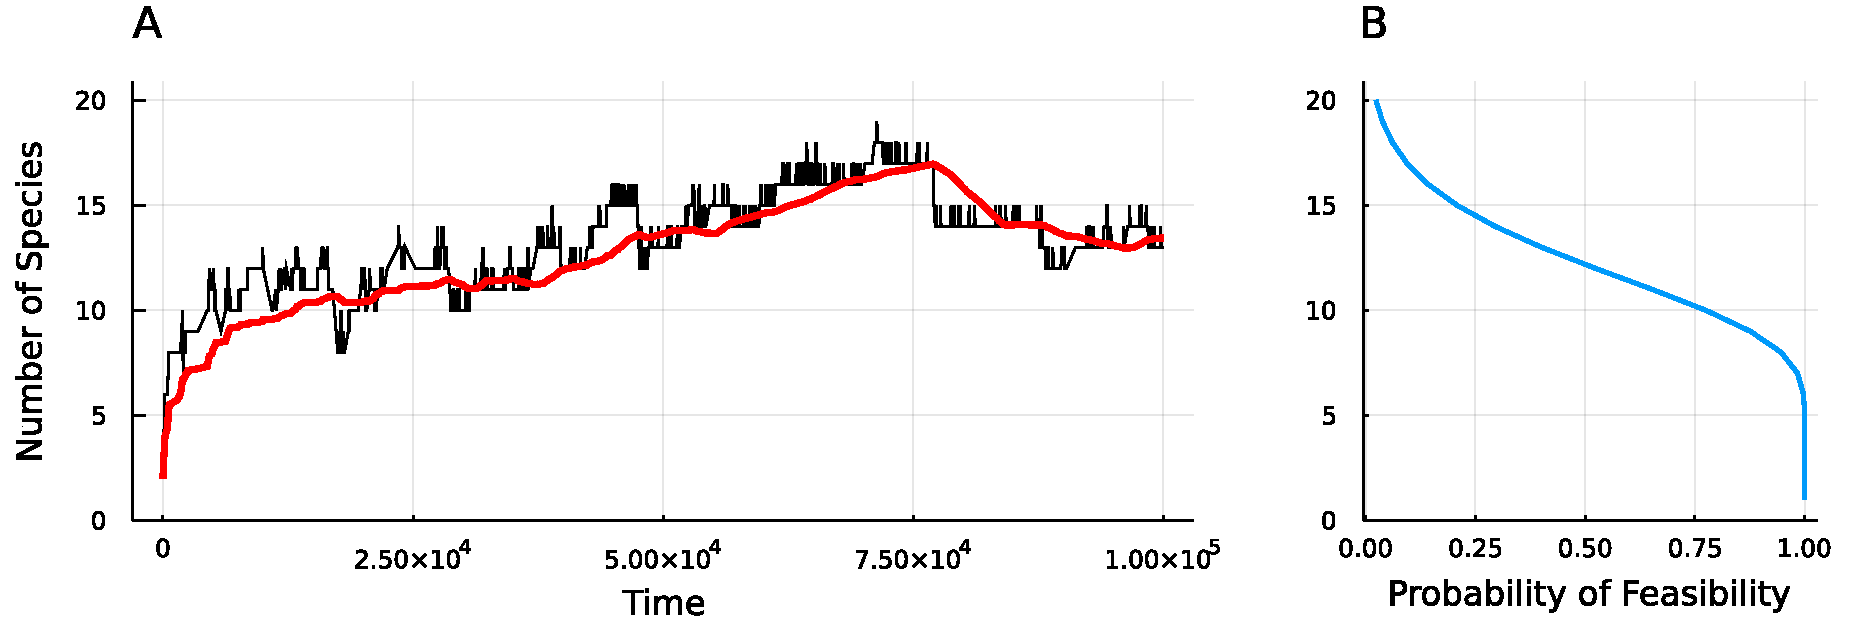
\includegraphics[width = \textwidth]{docs/Figures/Fig_3.pdf}
    \caption{Example of a single assembly trajectory (A) and the corresponding probability of feasibility vs species richness (B). (A) shows the species richness over time for a single assembling community simulated over \SI{1e5} time steps with species $\kappa$ and $a$ values drawn from the distributions X and X respectively . The black line shows the actual number of extant species in the system over time and the red the moving average (with a window $t = x$). (B) shows the probability of feasibility (\cref{EQ:P_feas_Temp}) plotted against species richness (on the y-axis) showing how the probability of a system being feasible falls as the number of species within increases. The species richness in (A) is seen to reach a relatively stable state at around $N = 15$, which corresponds to the point where the probability of feasibility is approaching $0$.   }
    \label{Fig:Assembly_Example}
\end{figure}

\section{Results}

\subsection{Feasibility is predicted well by the analytical bound}

To evaluate the analytical feasibility bound from \cref{EQ:Feas_sp} we numerically simulated randomly generated GLV systems with $N = 50$ and varying $\kappa$ and $\bar{a}$ values. For each of these systems we used \cref{EQ:Feas_sp} to predict if the systems would be feasible and compared this to the numerical simulations (where systems were unfeasible if any population went extinct). Overall \cref{EQ:Feas_sp} preformed well in predicting the feasibility of the randomly generated systems \cref{Fig:Feasability_Bound} with the minimum normalised carrying capacity required for feasibility increasing as interactions became more competitive \cref{Fig:Feasability_Bound}. We further demonstrate the generality of the \cref{EQ:Feas_sp} as a feasibility bound showing that it preforms well when varying the variance and distribution from which $a$ and $\kappa$ values are drawn from (\cref{SI_Sec:Feas_sims}). 

\begin{figure}[h] 
    \centering
    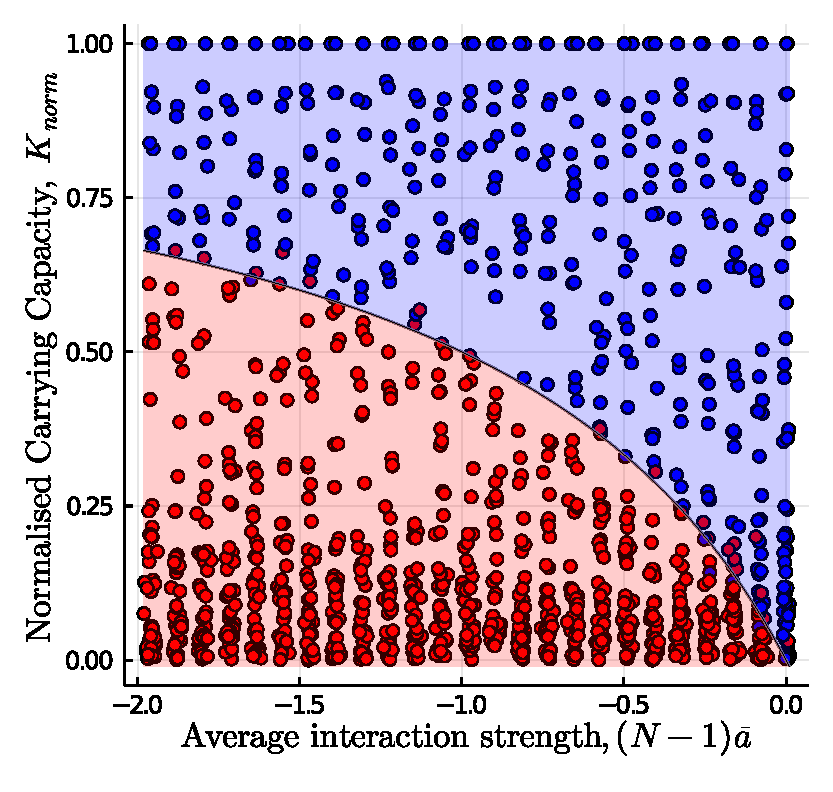
\includegraphics[width = 0.5\textwidth]{docs/Figures/Fig_1.pdf}
    \caption[width = \textwidth]{\textbf{Analytical predictions of feasibility} The theoretical bound (black line) gives the minimum value for $\kappa$ below which (area shaded in red) communities are unfeasible and above which (shaded blue) communities are expected to be feasible. Each point shown is the minimum $\kappa$ and average interaction strength value from a randomly generated community with $N=50$, simulated till equilibrium. Feasible systems (with no extinctions) are shown in blue and unfeasible systems in red. Overall the simulations match the expectations from \cref{EQ:Feas_sp} (i.e. the colours of the points and shaded areas match), predicting the feasibility of communities well.}
    \label{Fig:Feasability_Bound}
\end{figure}

\subsection{The distribution of thermal sensitivities ($E_a$)  determines the shape of the feasibility and species richness - temperature curve}

We looked at the effect of the distributions of thermal sensitivities $E$ on the shape of the the feasibility and species richness temperature responses. 

 Applying this approach to the distributions defined in \cref{EQ:Trait_distributions} we examine the effects of varying the distribution of thermal sensitivities on the temperature response species richness (as predicted by \cref{EQ:P_feas_Temp};\cref{fig:Nsp_Temp}). In doing so we can see that the distributions of thermal sensitives have the same qualitative effect as seen in \cref{EQ:Boltz_dist} with the average thermal response ($\mu_E$) determining the overall direction of the thermal response and the variance ($\sigma_E^2$) introducing curvature which creates a uni-modal shape.

\begin{figure}
    \centering
    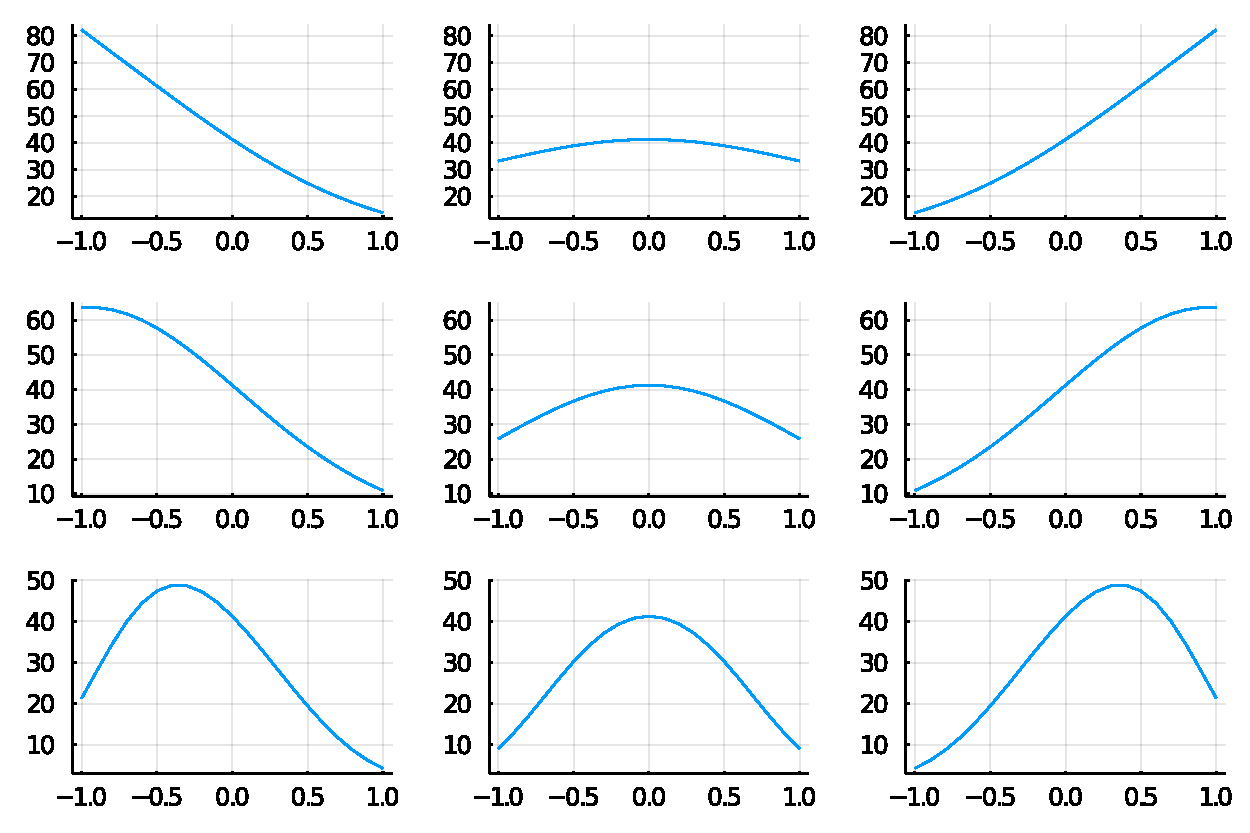
\includegraphics[width = \textwidth]{docs/Figures/Fig_Nsp_Temp.pdf}
    \caption{\textbf{\textit{(placeholder)} The effects of variation in $E_a$ on the thermal sensitivity of species richness.} The relationship between species richness and temperature changes depending on the shape of the distribution of thermal sensitivities of interaction strengths, $E_a$. Plots show the shape of the N vs T relationship as the average thermal sensitivity increases $\mu_{E_a}$ (panels a-c) and as variation in thermal sensitivity increases (as shown by coloured lines in each panel). Broadly, the direction of the response of richness to temperature is determined by the average $E_a$ value (panels a-c) whilst the presence/strength of the uni-modal relationship is determined by the variation in $E_a$ (colored lines) }
    \label{fig:Nsp_Temp}
\end{figure}

\subsection{The distribution of thermal sensitvties predictes the species richness of randomly assembled GLV communities}

\begin{figure}
    \centering
    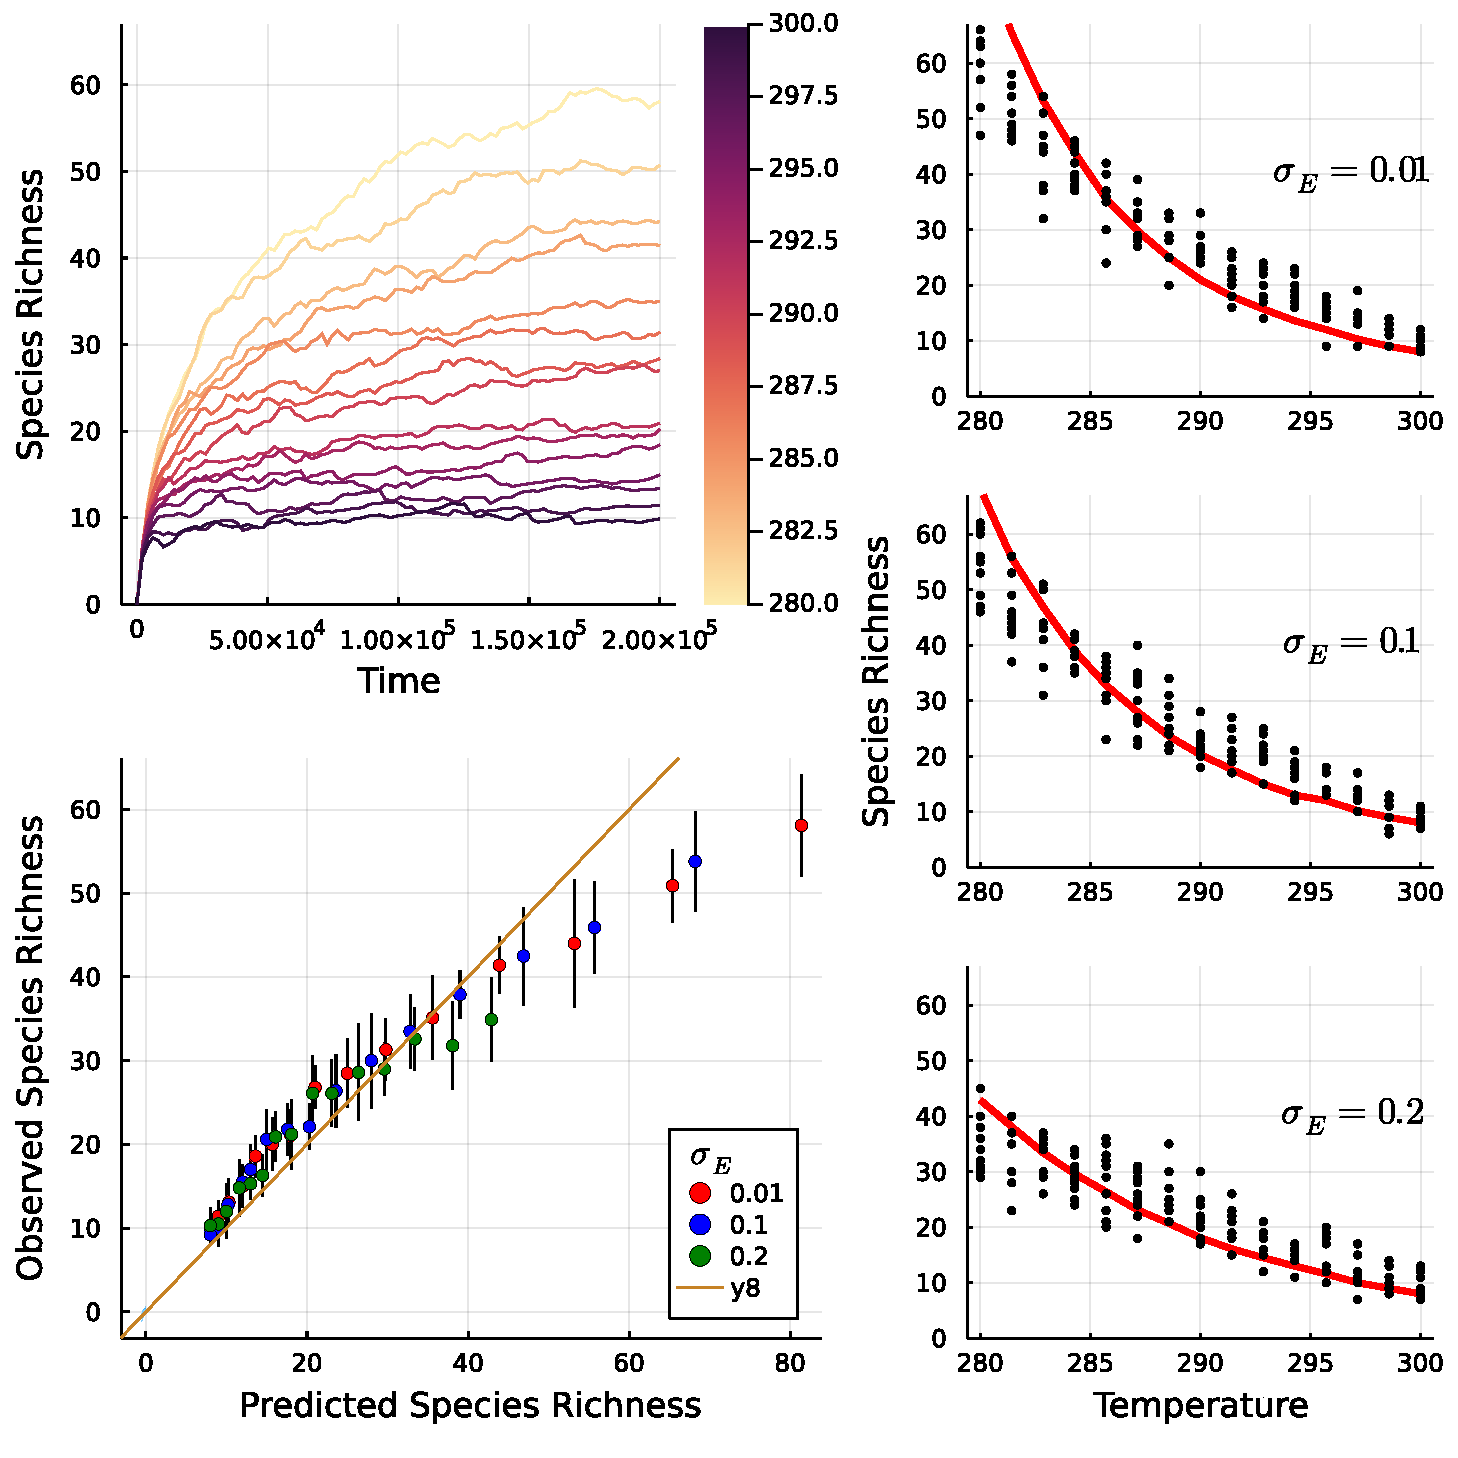
\includegraphics[width = \textwidth]{docs/Figures/Fig_4.pdf}
    \caption{Caption}
    \label{Fig:Temperature_assembly}
\end{figure}

\section{Supplementary Material}

\subsection{Mean-field approximation} \label{SI_Sec:Meanfield}

\subsection{Feasibility simulations} \label{SI_Sec:Feas_sims}

\subsection{Derivation of thermal response distributions} \label{SI_Sec:TPC_dist}


\end{document}
